\chapter{Prototype Screening Tool}
\label{ch:tool}

The two modules are integrated into an interactive, multi-page web application built with
Streamlit (\texttt{app/}). It runs locally on a laptop CPU; after a one-time start-up of about
40--60 seconds (loading the language model), each query is answered in a few seconds. The
interface was designed for non-specialists: every number carries a plain-language explanation,
a tooltip and, where relevant, a warning. It has four pages:

\begin{description}
  \item[Estimate a product] free-text query $\rightarrow$ estimate, range, confidence and explanation;
  \item[Recipe \& portfolio] bill-of-materials screening with hotspot detection;
  \item[How the model thinks] global explanations and validation results;
  \item[About \& how to use] a four-step guide, a glossary (CO\textsubscript{2}-eq, range, SHAP,
  match) and the limitations.
\end{description}

\section{Single-product mode}

Figure~\ref{fig:app1} shows the main page for the query ``frozen breaded chicken nuggets''. One-click
example queries help first-time users, and the query is kept in the page URL so a result can be
shared. The page follows the framework of Figure~\ref{fig:arch}:

\begin{enumerate}
  \item \textbf{Result card (Module A).} The XGBoost estimate (4.8~kg~\co/kg) is shown with its
  Mondrian-conformal 90\% range (2.4--9.6) and the expert value of the closest database product
  (3.87), which lies inside the range. Two badges translate the numbers for a lay reader: an
  \emph{impact level} (low / below average / above average / high, from database quartiles) and a
  \emph{confidence} level that combines the match similarity with the width of the range. A
  percentile bar places the product among all foods and within its food group.
  \item \textbf{``Why this number?'' (explainability).} A generated sentence names the main drivers
  (``pushed up by \emph{Meat, eggs, fish} ×1.69 and \emph{Chilled} ×1.20; pulled down by
  \emph{chicken} ×0.79''). A \emph{waterfall chart} then starts from the typical food in the database
  (3.02~kg~\co/kg, the SHAP base value) and applies each feature's multiplicative SHAP effect in turn
  until the final estimate is reached, so the explanation adds up exactly to the prediction. A
  caption reminds the user that SHAP explains the model, not physical causation.
  \item \textbf{Closest products (Module B).} The five most similar AGRIBALYSE entries are listed
  with their footprints and a similarity bar.
  \item \textbf{Where the footprint comes from.} The expert life-cycle stage breakdown of the closest
  product (farming, processing, packaging, transport, shop, home) is shown for context; it is
  labelled as descriptive, because these values are never model inputs.
  \item \textbf{Lower-impact similar options.} Products from the same sub-group with a footprint at
  least 30\% lower are suggested, ranked by similarity to the matched product; for meat products,
  plant-based substitutes are added (here, soybean-based nuggets, $-63\%$). This turns the estimate
  into an actionable comparison.
  \item \textbf{Editable attributes.} Food group, sub-group, storage, preparation, packaging data
  source, air-freight flag and ingredients are pre-filled from the best match and can be edited in a
  collapsible panel; the estimate and explanation update immediately, which supports ``what-if''
  exploration.
\end{enumerate}

\begin{figure}[ht]
\centering
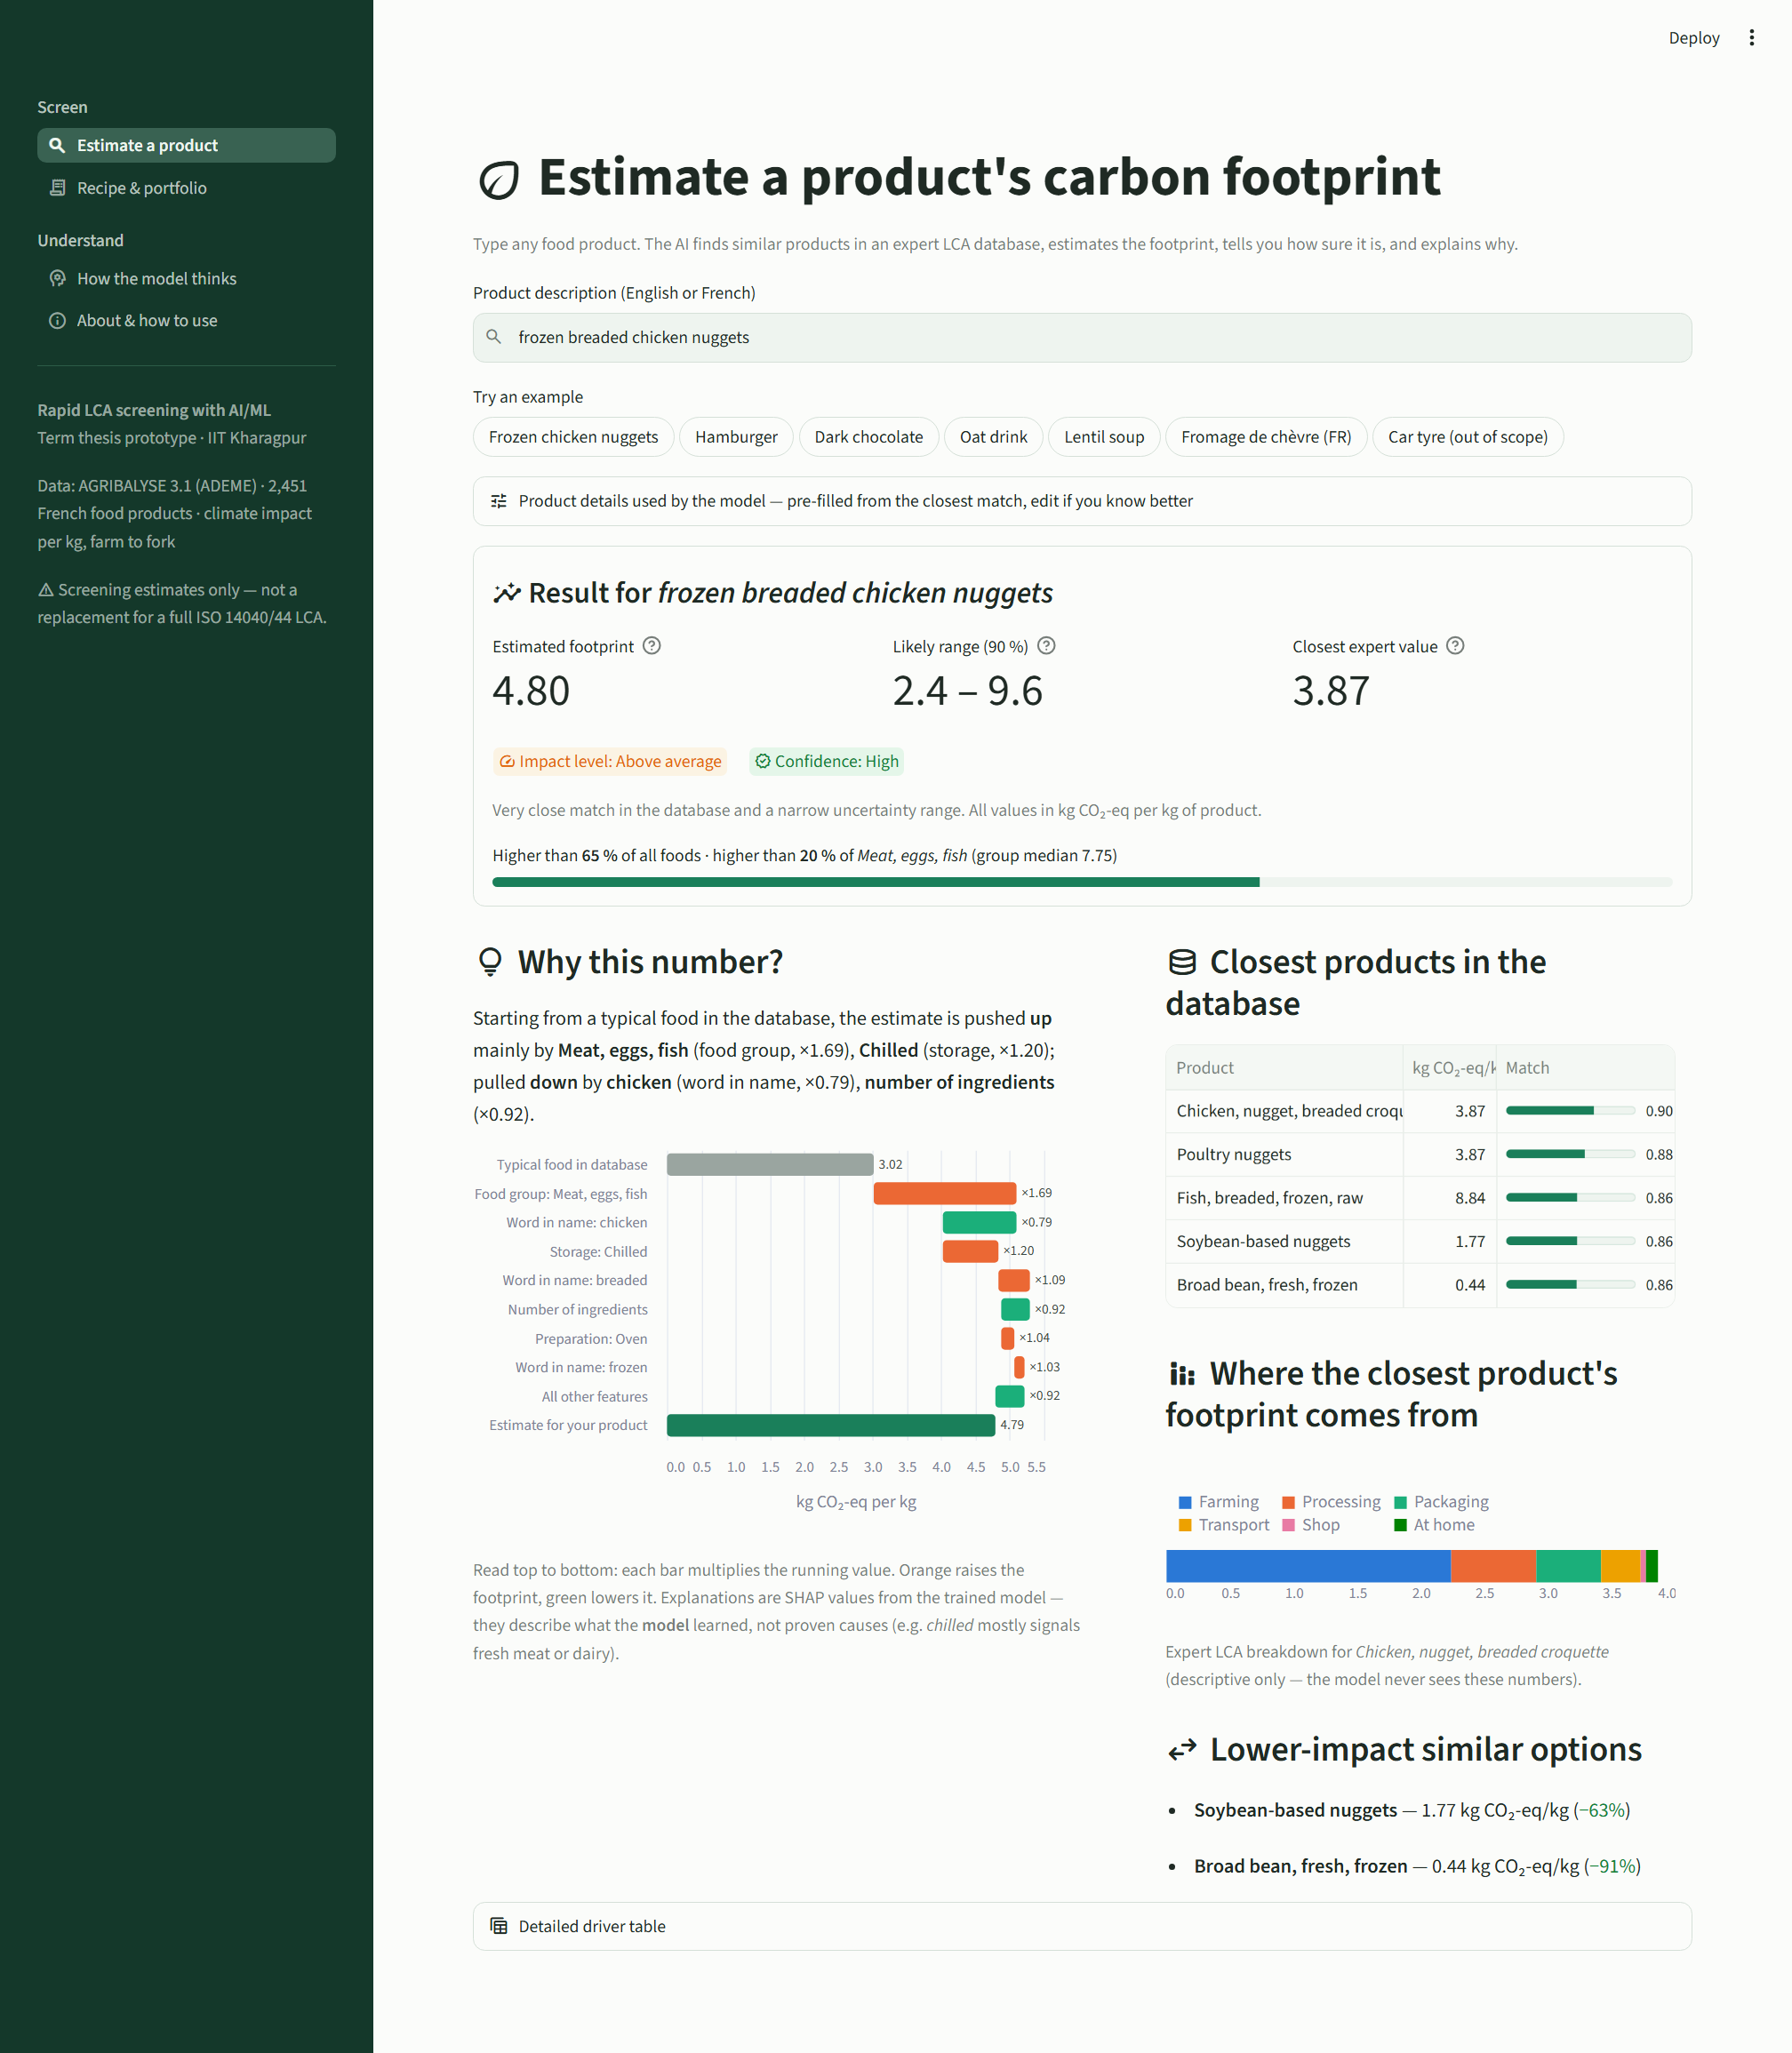
\includegraphics[width=\textwidth]{app_single}
\caption{Single-product screening for ``frozen breaded chicken nuggets'': result card with range, impact and confidence badges; waterfall explanation; closest datasets; stage breakdown of the closest product; and lower-impact alternatives.}
\label{fig:app1}
\end{figure}

\section{Applicability-domain warning}

For inputs outside the database's scope, nearest-neighbour retrieval still returns \emph{something};
without a guard, the user would receive a confident-looking but meaningless number. Figure~\ref{fig:app2}
shows the query ``car tyre'': the best similarity is 0.83, below the calibrated 0.85 threshold, so the
tool displays a prominent ``probably out of scope'' warning and the confidence badge drops to
\emph{Low}. This implements the recommendation of Song et al.\ \citep{song2017} that screening models
must state where they can be trusted.

The figure also shows \emph{why} the warning is essential. Behind it, the pipeline still produces
a plausible-looking number (6.0~kg~\co/kg, range 3.0--12.0), because the nearest dataset was a
pork product and the model faithfully estimates a pork product. The conformal interval cannot
detect this: it quantifies uncertainty \emph{within} the training distribution, not whether the
input belongs to it. Interval and applicability check are therefore complementary safeguards, and
neither can be dropped.

\begin{figure}[ht]
\centering
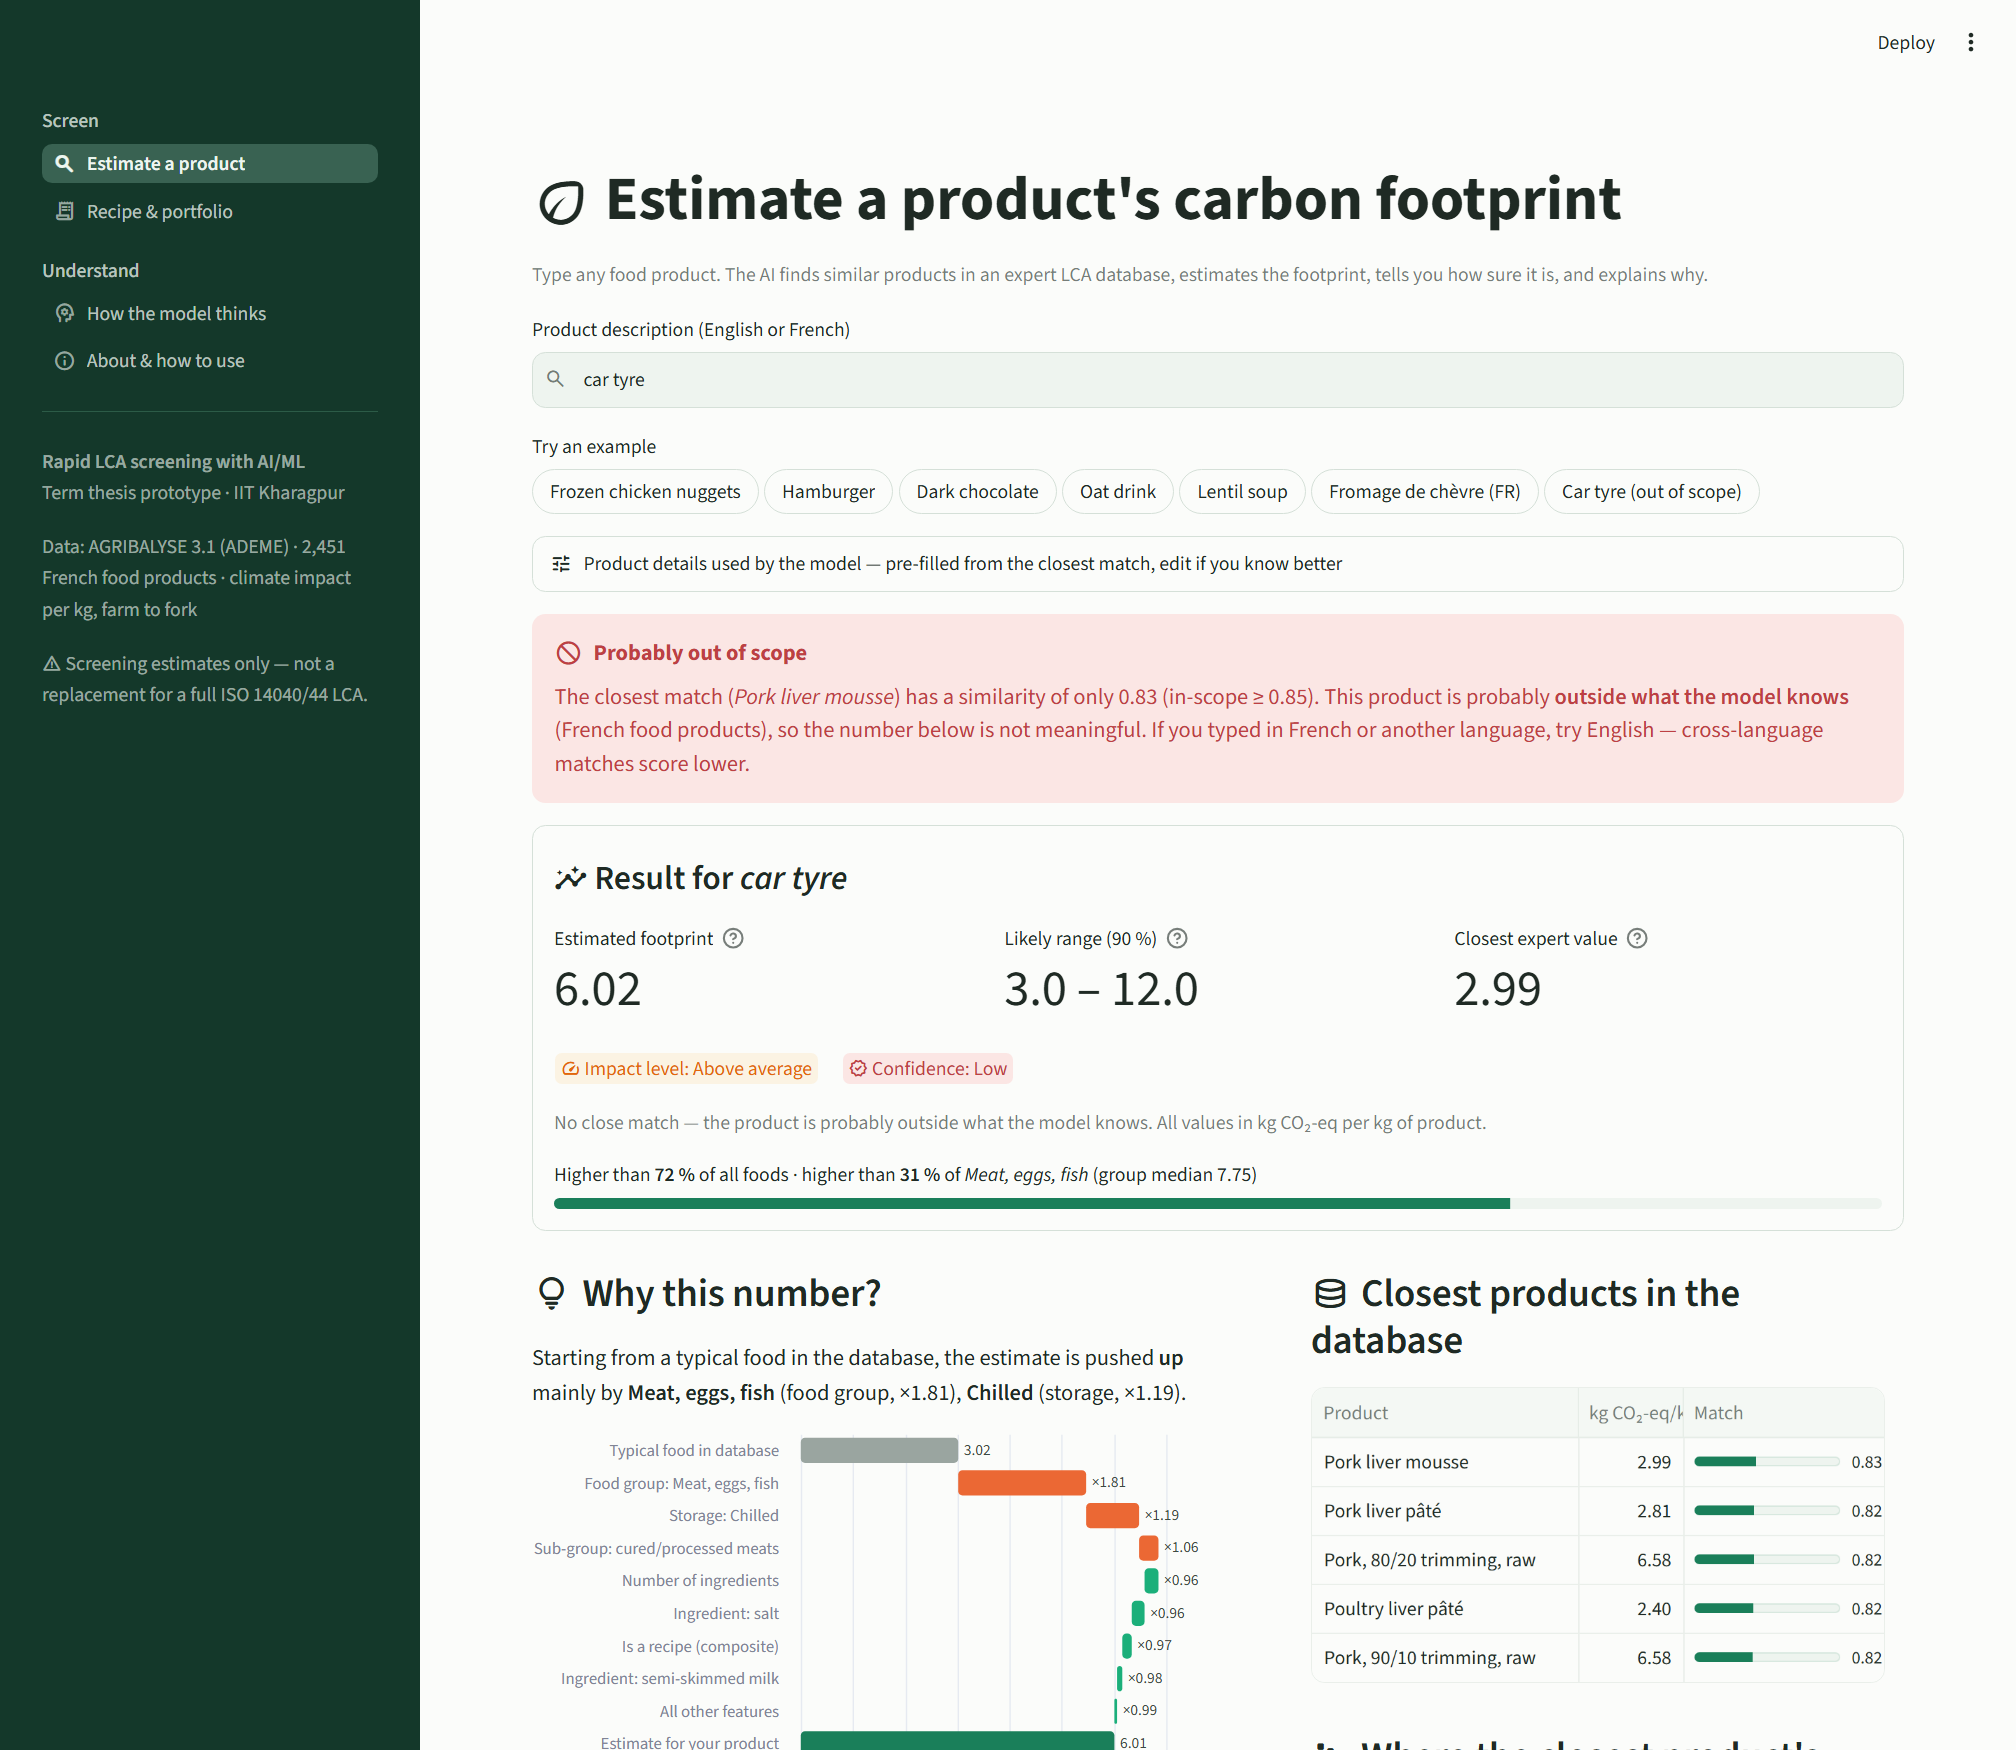
\includegraphics[width=0.9\textwidth, trim=0 0 0 0, clip]{app_ood}
\caption{Out-of-domain input (``car tyre''): low similarity triggers an explicit warning and a low-confidence badge.}
\label{fig:app2}
\end{figure}

\section{Recipe and portfolio mode}

The second page accepts an editable table of items and masses (e.g.\ 125~g minced beef, 150~g rice,
80~g tomato sauce, 30~g cheddar, 10~g olive oil). Each line is mapped, estimated and multiplied by
its mass. The page reports the total footprint, the biggest hotspot and its share, a ranked
contribution chart with the hotspot highlighted, per-item match quality, and lower-impact options
for the hotspot together with the saving each would bring to the recipe. In the example recipe,
minced beef contributes about 85\% of the total, and swapping it for soy-based mince would remove
most of the footprint. Low-similarity lines are flagged for manual review, results can be
downloaded as CSV, and item ranges are shown but not summed, because item errors are not
independent.

\section{Model insight page}

The ``How the model thinks'' page (Figure~\ref{fig:app3}) presents the global explanation and
validation evidence to users: headline metrics (91\% within a factor of two, $R^2=0.62$ on unseen
categories, 91\% interval coverage, 95\% top-5 matching), global SHAP importance, directional
effects of words and ingredients, an interactive comparison with the category-average shortcut
under both validation schemes, accuracy for six impact categories, and interval coverage by food
group, together with the honest caveat about new dairy sub-groups (Section~\ref{sec:e4}). This acts
as a built-in ``model card'', so users know the tool's intended use and failure modes.

\begin{figure}[ht]
\centering
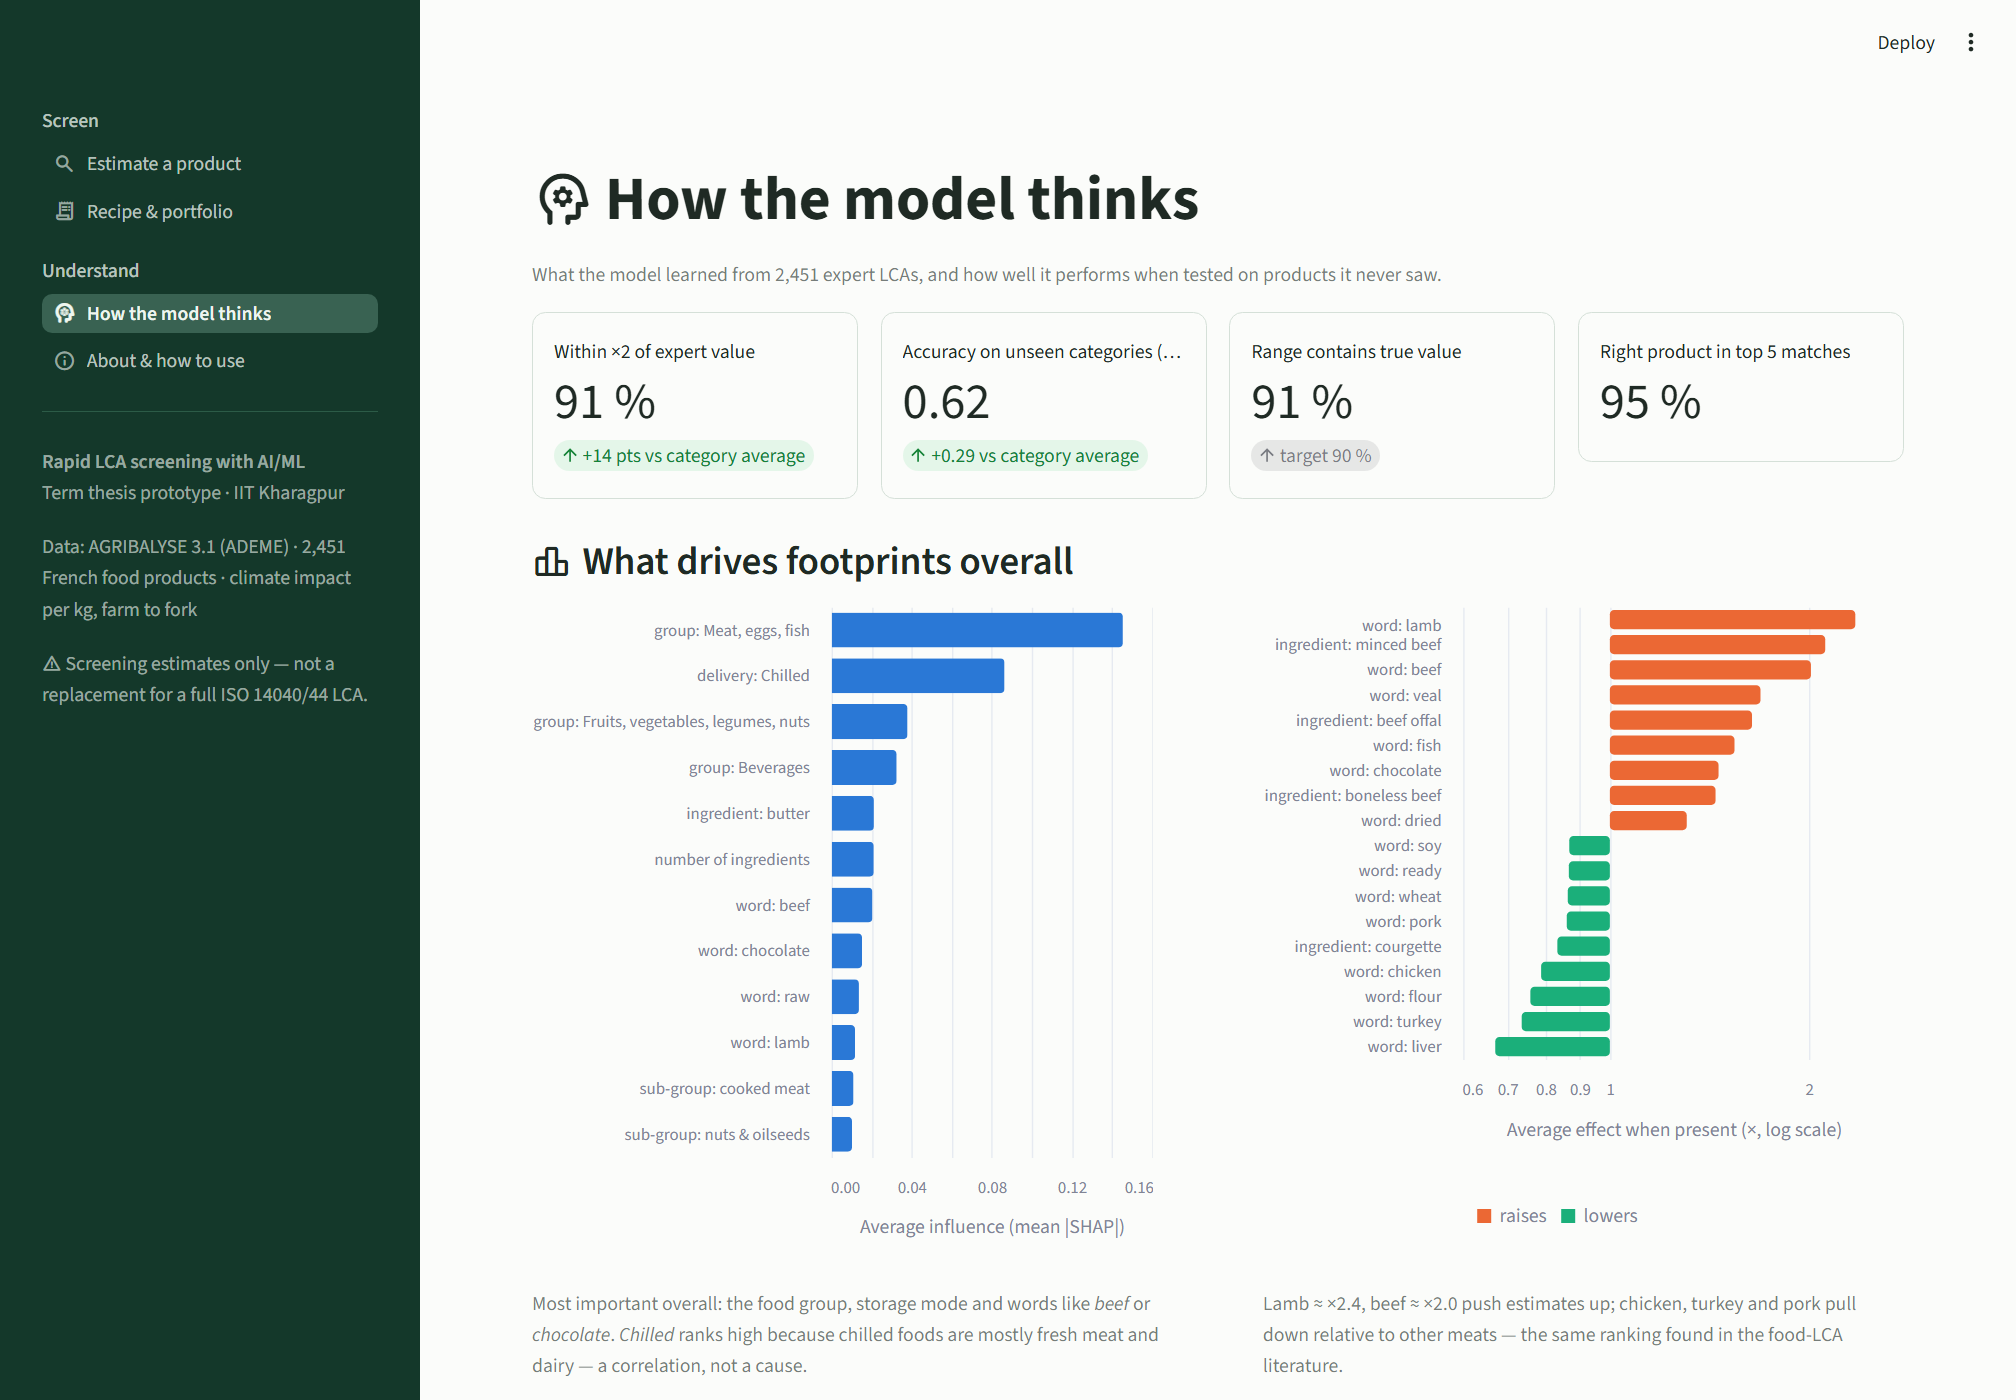
\includegraphics[width=\textwidth]{app_insights}
\caption{``How the model thinks'' page: headline validation metrics and global explanations.}
\label{fig:app3}
\end{figure}

\section{Intended use}

The tool is designed for \emph{screening}: prioritising which products, ingredients or suppliers
deserve a full LCA, comparing reformulation options early in design, and flagging likely hotspots
in large portfolios. It is \emph{not} intended to replace an ISO~14040/44 study, to produce EPDs,
or to support public comparative claims.
